\documentclass{ieeeojies}
\usepackage{cite}
\usepackage{amsmath,amssymb,amsfonts}
\usepackage{algorithmic}
\usepackage{graphicx}
\usepackage{textcomp}
\usepackage{amstext}
\graphicspath{{images/}}
\graphicspath{ {./images/} }
\usepackage{booktabs}
\usepackage{float}
\usepackage[table]{xcolor}
\usepackage{collcell}
\usepackage{hyperref}


\newcommand{\coloredcell}[1]{\cellcolor{red!10} #1}

\def\BibTeX{{\rm B\kern-.05em{\sc i\kern-.025em b}\kern-.08em
    T\kern-.1667em\lower.7ex\hbox{E}\kern-.125emX}}

\raggedbottom

\begin{document}
\title{Forecasting Vietnam Bank Stock Price by applying Machine Learning and Statistical models.}
\author{\uppercase{Ngo Manh Khuong (21522241)}\authorrefmark{1}, 
\uppercase{Ngo Cong Huan (21520881)\authorrefmark{2}, and Nguyen Thi Van Anh (21521835)}.\authorrefmark{3}
% \IEEEmembership{Member, IEEE} \textcolor{red}{(DO include authors from the first submission)}
}
\address[1]{University of Information Technology, Ho Chi Minh city (email: 21522241@gm.uit.edu.vn)}
\address[2]{University of Information Technology, Ho Chi Minh city (email: 21520881@gm.uit.edu.vn)}
\address[3]{University of Information Technology, Ho Chi Minh city (email: 21521835@gm.uit.edu.vn)}

% \tfootnote{This paragraph of the first footnote will contain support 
% information, including sponsor and financial support acknowledgment. For 
% example, ``This work was supported in part by the U.S. Department of 
% Commerce under Grant BS123456.''}

\markboth
{Author \headeretal: Khuong. Ngo Manh, Huan. Ngo Cong, Van Anh. Nguyen Thi.}
{Author \headeretal: Khuong. Ngo Manh, Huan. Ngo Cong, Van Anh. Nguyen Thi.}

\corresp{}

\begin{abstract}
In the context of the stock market, a share signifies a fraction of ownership in a company that is publicly traded. When a company opts to go public to raise funds, it splits its ownership into small, equal parts known as shares, which are then sold to investors on the stock market. The creation of dependable prediction models for the stock market enables investors to make more informed decisions. This study seeks to forecast the future stock prices of some major banks (ACB, VCB, BIDV) in Vietnam. Moreover, Machine Learning, which entails the development of computer tasks that mimic human intelligence, is currently the most widely used technique. It is presently a potent analytical tool for effectively managing investments in financial markets. The extensive application of machine learning in the financial sector has led to the emergence of a revolutionary method that can assist investors in making superior investment and management decisions to boost the performance of their securities assets. In this study, we initially examine the share prices of the aforementioned companies on the Vietnamese stock exchanges over the past five years. Subsequently, we utilize data and integrate some machine learning algorithms to predict future stock prices.
\end{abstract}

\begin{keywords}
Bank Stock Price Forecast, Linear Regression, ARIMA, SVR, Long Short-Term Memory (LSTM), Vector Autoregression (VAR), Random Forest, Seq2Seq, Fully Convolutional Neural Network (FCN)
\end{keywords}

\titlepgskip=-15pt

\maketitle

\section{Introduction}
\label{sec:introduction}
\hspace{1em}The accurate prediction of stock prices remains a critical challenge in financial markets, warranting continuous exploration and refinement of predictive models. In this paper, we undertake an in-depth analysis utilizing an array of forecasting models—ARIMA (AutoRegressive Integrated Moving Average), SVR (Support Vector Regression), LSTM (Long Short-Term Memory), Linear Regression, VAR (Vector Autoregression), Random Forest, Seq2Seq (Sequence-to-Sequence), FCN (Fully Convolutional Networks), alongside additional models—to forecast the stock prices of three prominent banks: ACB, VCB, and BIDV.

Stock markets exhibit a multifaceted nature, influenced by a multitude of internal and external factors, rendering the prediction of stock prices a complex endeavor. The inclusion of various models enables a holistic approach, accommodating diverse perspectives and capturing intricate patterns within the stock market data. Each model contributes distinct capabilities and intricacies, facilitating a comprehensive understanding of the underlying trends and dynamics governing the stock prices of these major banking institutions.

Throughout this study, we aim to not only assess the predictive accuracy but also to compare the robustness and reliability of these diverse forecasting models. Metrics such as Root Mean Squared Error (RMSE), Mean Absolute Percentage Error (MAPE), and Mean Squared Logarithmic Error (MSLE) will be employed for a comprehensive evaluation of model performance. By examining these metrics, we seek to offer insights into the strengths and limitations of each model in the context of stock price prediction for ACB, VCB, and BIDV.

The significance of comprehending the nuances of stock price forecasting, coupled with the evaluation of multiple predictive models using diverse performance metrics, cannot be overstated. This paper strives to contribute to the ongoing discourse in financial market analysis by presenting a rigorous evaluation of various models, thus facilitating a deeper understanding of the complexities inherent in stock market dynamics.

Understanding the comparative performance of these models in terms of RMSE, MAPE, and MSLE metrics is instrumental for investors in making informed decisions and for researchers and practitioners in enhancing the precision and reliability of financial market predictions. By critically examining these models' performances, this study aims to provide valuable insights into optimizing investment strategies and fostering well-informed financial decision-making.

This paper serves as a comprehensive exploration of diverse predictive models applied to the stock prices of significant banking entities, paving the way for further advancements in the field of financial market analysis and forecasting.


\section{RELATED WORK}
\hspace{1em}Vaishnavi Gururaj and his team from Global Academy of Technology, Bengaluru, India apply Linear Regression (LR) to easily available sample data, followed by observations. Subsequently, Support Vector Regression (SVR) is employed, and observations and results are graphically plotted. Support Vector Machines (SVMs), with advanced features like high accuracy and predictability, are introduced for comparison. The survey of pros and cons for both techniques leads to the conclusive finding that SVM outperforms LR in predicting values.\cite{a1}

Prapanna Mondal , Labani Shit and Saptarsi Goswami conducted a study on fifty six stocks from seven sectors Accuracy of ARIMA model in predicting stock prices is above 85\%, which indicates that ARIMA gives good accuracy of prediction.\cite{a2}

Bruno Miranda Henrique from The Journal of Finance and Data Science SVR to evaluate its performance on a range of Brazilian, American, and Chinese stocks with varying attributes, such as small-cap or blue-chip stocks. This research demonstrates that when utilizing a linear kernel with a fixed training set of daily prices, it is possible to get reduced prediction errors in the test set compared to the training set. Furthermore, with daily prices and fixed training models, this kernel performed better for price predictions than the radial and polynomial kernels. Nevertheless, employing a fixed training time decreased the model's predictive effectiveness when the price frequency was increased to minutes. Specifically, for nearly all stocks examined in real-time prices, SVR yielded less accurate predictions than a random walk model when employing fixed training.\cite{a3}

Computer Science Department, School of Computer Science, Bina Nusantara University, Jakarta, 11480, Indonesia developed LSTM program using Python and Tensorflow for stock prices prediction (accuracy 94.59\% at 100 epoch). Comparing with other research for stock price forecasting, LSTM method is better (usually neural network method only about 90\% accuracy).\cite{a4}

Phillip Hushani uses VAR model to make predictions using the NASDAQ closing price. Based on these experiments, a medium-term trading strategy has been developed. The analysis shows that the LSTM is the most accurate model. The VAR model can predict the trend more accurately than the other models.\cite{a5}

The results of this study revealed that the Random Forest (RF) algorithm has the best accuracy because it received a 94.12\% accuracy ratio in this work. They worked on the choice of advantage, the advantages of classifying the basic advantage,and how to use new techniques to predict the best field in the stock market.\cite{a6}

Soonsung Hwang and his colleagues performed an experiment on Temperature Prediction in Firing Furnace Process. The proposed model shows very high accuracy in predicting the future temperature of the kiln, outperforming other baseline models. This shows that the Seq2Seq model has the ability to predict with high accuracy rate with time series data.\cite{a7}

Jizhong Wu researches a fully convolutional network (FCN)-based fault detection method to segment seismic images and identify faults. The results of the study show that the FCN model shows more accurate and effective error detection than traditional methods, with fast prediction time and high accuracy.\cite{a8}

\section{MATERIALS AND METHODS}
\subsection{Data collection}
\hspace{1em}We use Vietnam bank stock price (ACB, BIDV, VCB) from \href{https://www.investing.com}{investing.com} website. Each dataset range from 22/12/2013 to 22/12/2023, and contains following columns:
\begin{itemize}
    \item Date: stock trading opening day. 
    \item Price (also known as Close Price): the last price at which 
a stock trades upon the end of the exchange. 
    \item Open: the first price at which a stock opens for trading. 
    \item High: highest stock price of the day. 
    \item Low: lowest stock price of the day. 
    \item Volume: the number of shares that the trader buys and 
sells. 
    \item Change: today's change in stock price from the previous 
day is expressed as a percentage
\end{itemize}
\subsection{descriptive statistic}
\begin{table}[H]
    \centering
    \begin{tabular}{|c|c|c|c|}
    \hline
     & \cellcolor{blue!10}\textbf{ACB} & \cellcolor{blue!10}\textbf{VCB} & \cellcolor{blue!10}\textbf{BIDV} \\
    \hline
    \cellcolor{blue!10}\textbf{Count}  & 2493 & 2496 & 2472\\ 
    \hline
    \cellcolor{blue!10}\textbf{Median}  & 11285.2 & 48528 & 26021.7\\
    \hline
    \cellcolor{blue!10}\textbf{Mean} & 13078.93 & 50337.02 & 25255.92\\
    \hline
    \cellcolor{blue!10}\textbf{Std}   & 7898.92 &26073.23  & 11804.1\\
    \hline
    \cellcolor{blue!10}\textbf{Variance}  & 62393053.17 & 679813431 &139336897.2 \\
    \hline
    \cellcolor{blue!10}\textbf{Deviation Coefficient}    & 0.603 & 0.517 & 0.467\\
    \hline
    \cellcolor{blue!10}\textbf{Skewness}   & 0.515 & 0.127 & 0.144\\
    \hline
    \cellcolor{blue!10}\textbf{Kurtosis}  & -1.158 & -1.366 & -1.257\\
    \hline
    \cellcolor{blue!10}\textbf{Min}   & 3885.1 & 10477 & 8006.4\\
    \hline
    \cellcolor{blue!10}\textbf{25\%}   & 5279.7 & 26196 & 12801.725\\
    \hline
    \cellcolor{blue!10}\textbf{50\%}   & 11285.2 & 48528 & 26021.7\\
    \hline
    \cellcolor{blue!10}\textbf{75\%}   & 21700 & 75174 & 34273.525\\
    \hline
    \cellcolor{blue!10}\textbf{Max}  & 30360 & 106500 & 49100\\
     \hline
    \end{tabular}
    \caption{Descriptive Statistic}
    \label{Descriptive Statistics}
\end{table}
\begin{figure}[H]
    \centering
    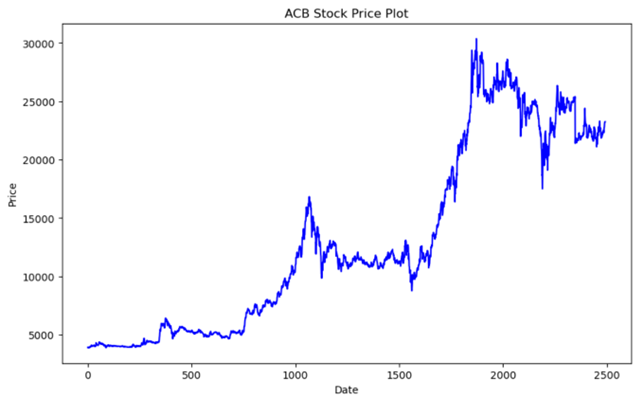
\includegraphics[width=1\linewidth]{ACB_plot.png}
    \caption{ACB stock price box plot}
    \label{fig:enter-label}
\end{figure}
\begin{figure}[H]
    \centering
    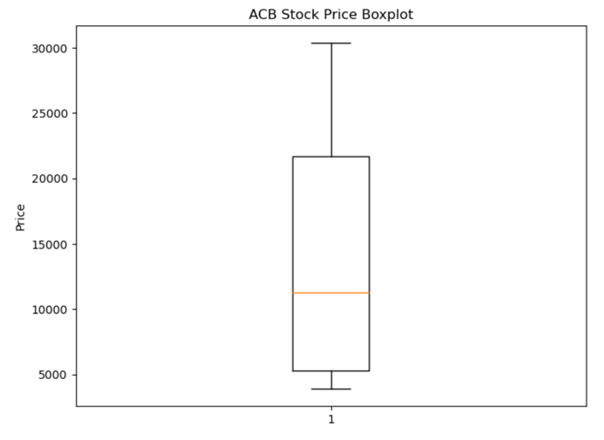
\includegraphics[width=1\linewidth]{ACB_boxplot.png}
    \caption{ACB stock price box plot}
    \label{fig:enter-label}
\end{figure}
\begin{figure}[H]
    \centering
    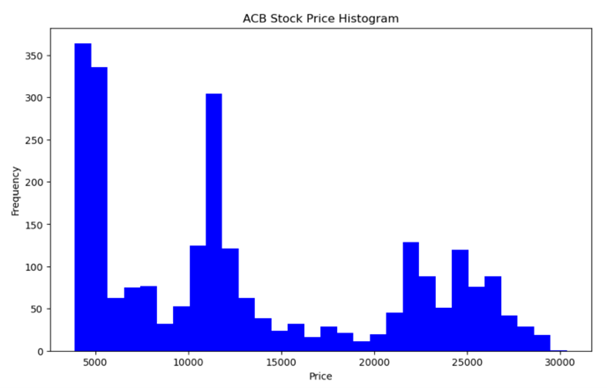
\includegraphics[width=1\linewidth]{ACB_histogram.png}
    \caption{ACB stock price histogram plot}
    \label{fig:enter-label}
\end{figure}

\begin{figure}[H]
    \centering
    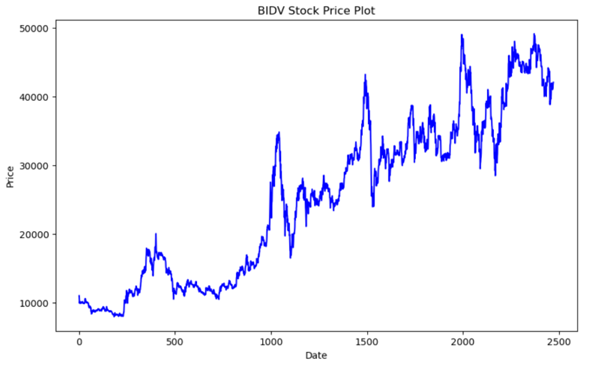
\includegraphics[width=1\linewidth]{BIDV_plot.png}
    \caption{BIDV stock price plot}
    \label{fig:enter-label}
\end{figure}
\begin{figure}[H]
    \centering
    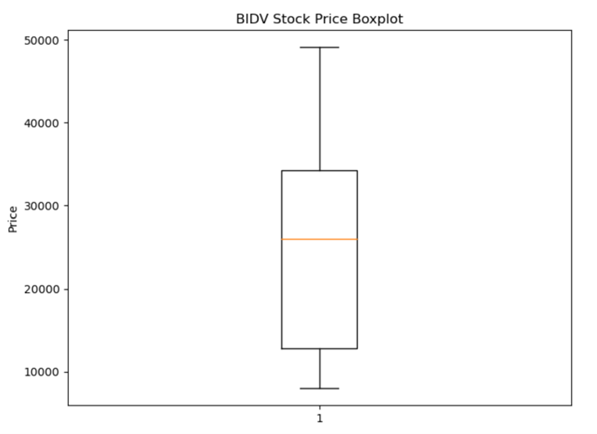
\includegraphics[width=1\linewidth]{BIDV_box.png}
    \caption{BIDV stock price box plot}
    \label{fig:enter-label}
\end{figure}
\begin{figure}[H]
    \centering
    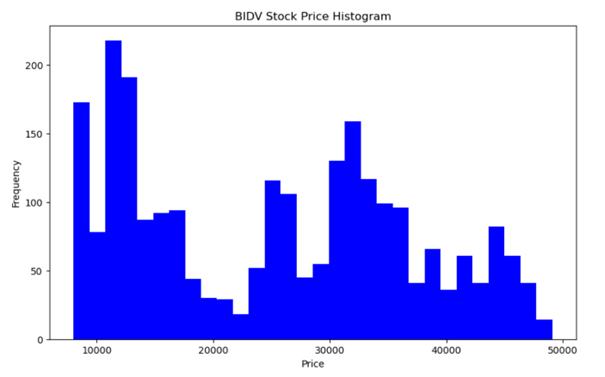
\includegraphics[width=1\linewidth]{BIDV_histogram.png}
    \caption{BIDV stock price histogram plot}
    \label{fig:enter-label}
\end{figure}
\begin{figure}[H]
    \centering
    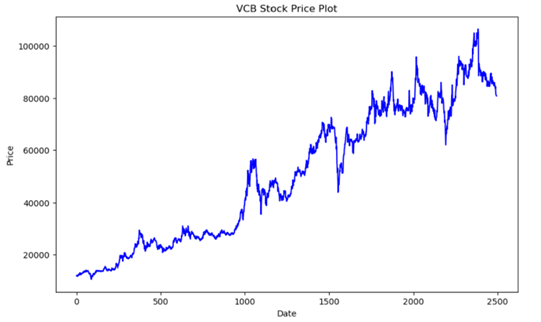
\includegraphics[width=1\linewidth]{VCB_plot.png}
    \caption{VCB stock price plot}
    \label{fig:enter-label}
\end{figure}
\begin{figure}[H]
    \centering
    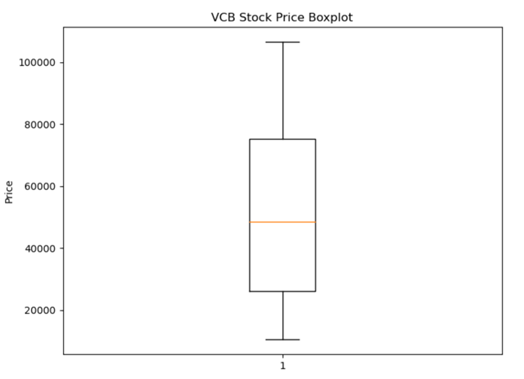
\includegraphics[width=1\linewidth]{VCB_box.png}
    \caption{VCB stock price box plot}
    \label{fig:enter-label}
\end{figure}
\begin{figure}[H]
    \centering
    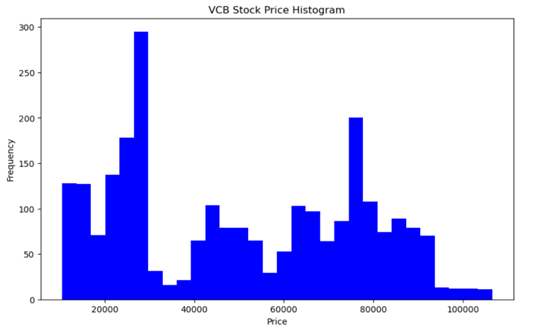
\includegraphics[width=1\linewidth]{VCB_histogram.png}
    \caption{VCB stock price histogram plot}
    \label{fig:enter-label}
\end{figure}
\subsection{algorithms}
\hspace{1em}The picture below shows how we perform algorithms in this report.
\begin{figure}[H]
    \centering
    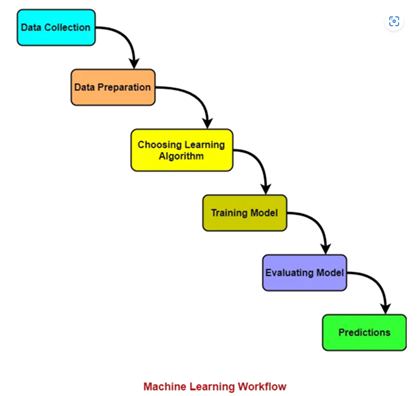
\includegraphics[width=0.75\linewidth]{workflow.png}
    \caption{Workflow of performing Machine learning}
    \label{fig:enter-label}
\end{figure}
\subsubsection{\textbf{Linear Regression}}
\hspace{1em}Linear Regression Model is a statistical model that describes the linear relationship between a response variable Y and multiple predictor variables $X_1,..., X_p$ ., where Y is linearly dependent on X.\cite{a9}
\\Important terms:
\[Y = b_0 + b_1 X_1 + b_2 X_2 + ... + bp Xp + e\]
where:
\begin{itemize}
    \item \textbf{Dependent variable Y}: The variable that is being predicted. In other words, Y is the variable whose value we are trying to determine based on the value of X.
    \item \textbf{Independent variable $X_1,X_2,...X_p$}: The variable that is used to predict Y. In other words, X is the variable whose value we know, and we are using that value to estimate the value of Y.
    \item \textbf{Intercept $b_0$}: The value of Y when X is 0. In other words, b0 is the value of Y when there is no relationship between X and Y.
    \item \textbf{Slope $b1,b2,..,bp$}: The rate of change of Y with respect to X. In other words, b1 indicates how much Y changes when X changes by one unit.
\end{itemize}

\subsubsection{\textbf{ARIMA}}
\hspace{1em}ARIMA is commonly used for forecasting time series data that exhibit trends, seasonality, and other temporal patterns. They are versatile and can be applied to various domains such as finance, economics, weather forecasting, and more. ARIMA consists of three components:
\begin{itemize}
    \item \textbf{AutoRegressive}: AR(p) is a regression model with lagged values of y, until p-th time in the past, as predictors. Here, p = the number of lagged observations in the model, $\epsilon$ is white noise at time t, c is a constant and $\phi$s are parameters.
    \[y_t = c + \phi_1 y_{t-1} + \ldots + \phi_p y_{t-p} + \varepsilon_t\]
    \item \textbf{Integrated I(d)}: The difference is taken d times until the original series becomes stationary. A stationary time series is one whose properties do not depend on the time at which the series is observed.
    
    \item \textbf{Moving average MA(q)}:  A moving average model uses a regression like model on past forecast errors. Here, $\epsilon$ is white noise at time t, c is a constant, and $\phi$s are parameters
    \[y_t = c + \theta_1 \varepsilon_{t-1} + \ldots + \theta_q \varepsilon_{t-q}\]
\end{itemize}
Combining all of the three types of models above gives the resulting ARIMA(p,d,q) model: \cite{a10}
\[Y_t = c + \phi_1 Y_{t-1} + \ldots + \phi_p Y_{t-p} + \theta_1 \varepsilon_{t-1} + \ldots + \theta_q \varepsilon_{t-q} + \varepsilon_t\]

where:
\begin{align*}
  Y_t & \text{ is the value of the time series at time } t, \\
  c & \text{ is a constant term,} \\
  \phi_1,.., \phi_p & \text{ are the autoregressive parameters,} \\
  \varepsilon_t & \text{ is the white noise term at time } t, \\
  \theta_1,.., \theta_q & \text{ are the moving average parameters,} \\
  p & \text{ is the order of the autoregressive part, and} \\
  q & \text{ is the order of the moving average part.}
\end{align*}

\subsubsection{\textbf{Support Vector Regression (SVR)}}
\hspace{1em}Support Vector Regression (SVR) is an extension of the Support Vector Machine (SVM) technique. Researchers have found that SVM provides excellent performance in time series forecasting. SVM finds an optimal hyperplane to separate two classes of samples. SVR finds an optimal hyperplane in high-dimensional space to separate data samples and minimize prediction error.

The SVR optimization function formula, with w being the unknown parameter vector: \cite{a11}
\begin{equation}
\begin{aligned}
& \underset{w, b, \zeta, \zeta^*}{\text{min}}
& & \frac{1}{2} \|w\|^2 + C \sum_{i=1}^{n} (\zeta_i + \zeta_i^*) \\
& \text{subject to}
& & y_i - (w \cdot \phi(x_i) + b) \leq \varepsilon + \zeta_i, \quad i = 1, \ldots, n \\
& & & (w \cdot \phi(x_i) + b) - y_i \leq \varepsilon + \zeta_i^*, \quad i = 1, \ldots, n \\
& & & \zeta_i, \zeta_i^* \geq 0, \quad i = 1, \ldots, n
\end{aligned}
\end{equation}

Two common kernels used in SVR include:
Radial Basis Function (RBF) Kernel:
\[K(x_i, x_j) = \exp\left(-\frac{\|x_i - x_j\|^2}{2\sigma^2}\right)\]
Polynomial Kernel:
\[K(x_i, x_j) = (\gamma x_i \cdot x_j + r)^d\]

\subsubsection{\textbf{Long Short-Term Memory (LSTM)}}
\hspace{1em}Long Short-Term Memory (LSTM) is an improvement from the RNNs, which is able to solve the Gradient Problem. The LSTM models essentially extend the RNN's memory to enable them to keep and learn long-term dependencies of inputs.\cite{a12}. A typical LSTM block is configured mainly by memory cell state, forget gate, input gate, and output gate. The crucial element, memory cell state, runs down through the entire chain to selectively add or remove information to the cell state with the help of the three gates.\cite{a13}

\begin{figure}[h!]
    \centering
    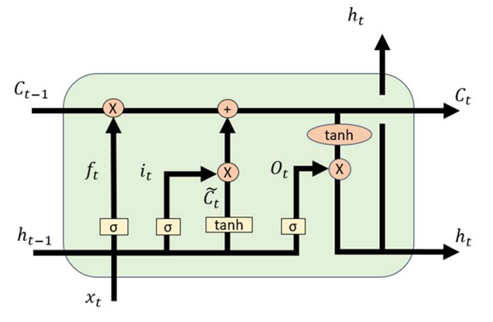
\includegraphics[width=0.75\linewidth]{LSTM_cell.png}
    \caption{A single LSTM cell}
    \label{fig:enter-label}
\end{figure}

Formulas for each LSTM cell:
\begin{align*}
i_t &= \sigma(W_{ii}x_t + b_{ii} + W_{hi}h_{t-1} + b_{hi}) \\
f_t &= \sigma(W_{if}x_t + b_{if} + W_{hf}h_{t-1} + b_{hf}) \\
o_t &= \sigma(W_{io}x_t + b_{io} + W_{ho}h_{t-1} + b_{ho}) \\
g_t &= \tanh(W_{ig}x_t + b_{ig} + W_{hg}h_{t-1} + b_{hg}) \\
c_t &= f_t \odot c_{t-1} + i_t \odot g_t \\
h_t &= o_t \odot \tanh(c_t)
\end{align*}
Where:
\begin{itemize}
    \item \(x_t\) is the input at time \(t\).
    \item \(h_{t-1}\) is the hidden state from the previous time step.
    \item \(i_t\), \(f_t\), \(o_t\), and \(g_t\) are the input, forget, output, and cell input vectors, respectively.
    \item \(W\) and \(b\) are weight and bias matrices.
    \item \(\sigma\) is the sigmoid activation function.
    \item \(\odot\) denotes element-wise multiplication.
\end{itemize}

\subsubsection{\textbf{Vector Autoregression (VAR)}}
\hspace{1em}Christopher Sims (1980) provided a new macroeconometric framework that held great promise: vector autoregressions (VARs). A univariate autoregression is a single-equation, single-variable linear model in which the current value of a variable is explained by its own lagged values. A VAR is an n-equation, n-variable linear model in which each variable is in turn explained by its own lagged values, plus current and past values of the remaining n-1 variables.

VAR is a forecasting algorithm that can be used when two or more time series influence each other, i.e. the relationship between the time series involved is bidirectional.\cite{a14}

The VAR(p) model of order p can be represented in the following formula: \cite{a15}
\begin{equation}
    Y_{1} = C + A_{1,1}Y_{1}^{(1)} + A_{1,2}Y_{1}^{(2)} + \ldots + A_{1,n}Y_{1}^{(n)} + E_{1}
\end{equation}

Where:
\begin{itemize}
    \item \( Y_{1} \) is the main variable.
    \item \( C \) is a constant.
    \item \( A_{1,1}, A_{1,2}, \ldots, A_{1,n} \) are coefficients.
    \item \( Y_{1}^{(1)}, Y_{1}^{(2)}, \ldots, Y_{1}^{(n)} \) are related variables.
    \item \( E_{1} \) is an error term.
\end{itemize}


\textbf{Steps that we need to follow to build the VAR model are:} \\
1. Examine the Data \\
2. Test for stationarity\\
2.1 If the data is non-stationary, take the difference.\\
2.2 Repeat this process until you get the stationary data.\\
3. Train/Test Split\\
4. Grid search for order P\\
5. Apply the VAR model with order P\\
6. Forecast on new data.\\
7. If necessary, invert the earlier transformation.

\subsubsection{\textbf{Random Forest}}
\hspace{1em}Random forests are a machine learning model that combines multiple decision trees to produce more accurate and robust results than a single tree. They work by using the idea of "wisdom of the crowds", in which many simple models can make more accurate predictions than a more complex model.\cite{a9}

\textbf{Random forests work in four steps:}
\\1.	Randomly select samples from the given dataset.
\\2.	Build a decision tree for each sample and get the prediction results from each decision tree.
\\3.	Take a vote for each prediction result.
\\4.	Choose the most predicted result as the final prediction.

Decision trees are simple machine learning models that can be used for classification or forecasting tasks. They work by splitting the data into branches based on certain features. Random forests use multiple decision trees to produce more accurate results.
\begin{enumerate}
    \item For \(k = 1\) to \(K\):
    \begin{itemize}
        \item Sample a bootstrap sample from the training data.
        \item Train a decision tree \(T_k\) on the bootstrap sample.
    \end{itemize}
    \item For a new input \(X\):
    \begin{itemize}
        \item For each tree \(T_k\), obtain the prediction \(Y_k\).
        \item Aggregate predictions: \( \hat{Y} = \frac{1}{K} \sum_{k=1}^{K} Y_k \) (for regression) or \( \hat{Y} = \text{mode}(Y_1, Y_2, \ldots, Y_K) \) (for classification).
    \end{itemize}
\end{enumerate}

\subsubsection{\textbf{Seq2Seq}}
\hspace{1em}The seq2seq model is a deep learning neural network architecture used in natural language processing and tasks involving sequential data. It consists of two main parts are encoder and decoder. \\
\textbf{Encoder:}
\begin{itemize}
    \item \textbf{Input:} Input sequence $x = (x_1, x_2, \dots, x_t)$
    \item \textbf{Context representation:} The hidden state of the LSTM is computed as $h_t = \text{LSTM}(x_t, h_{t-1})$
\end{itemize}

\textbf{Decoder:}
\begin{itemize}
    \item \textbf{Output:} Output sequence $y = (y_1, y_2, \dots, y_t')$
    \item \textbf{Initial state:} $(s_0)$ is initialized from $h_t$
    \item \textbf{Update hidden state:} $s_t = \text{LSTM}(y_t, s_{t-1})$
    \item \textbf{Output prediction:} $P(y_t|y_{<t}, x) = \text{softmax}(W_{\text{out}} s_t + b_{\text{out}})$
\end{itemize}

\textbf{Training:}
\begin{itemize}
    \item \textbf{Loss function:} $L(y, y') = -\frac{1}{T'} \sum_{t=1}^{T} \log P(y_t|y_{<t'}, x)$
    \item Parameters are updated using backpropagation and optimization algorithms (e.g., SGD, Adam)
\end{itemize}

\subsubsection{\textbf{Fully Convolutional Neural Network (FCN)}}
\hspace{1em}FCNs (Fully Convolutional Neural Networks) were introduced by Wang et al. (2017b) for classifying time series. They lack local pooling layers, maintaining the time series length during convolutions. FCNs use a Global Average Pooling (GAP) layer instead of a final FC layer, reducing parameters and enabling the identification of crucial segments contributing to classifications via Class Activation Mapping (CAM). The architecture includes three convolutional blocks with batch normalization and ReLU activation. FCNs exhibit parameter invariance in most layers across time series lengths, facilitating transfer learning.\cite{a16}

\[conv(i,j) = R( \sum_{u=0}^{M-1} \sum_{v=0}^{M-1} w_{u,v} x_{i+u,j+v} +b)\]

Where:
\begin{itemize}
    \item \( \text{conv}(i, j) \) represents the convolution operation at position \((i, j)\).
    \item \( R \) is an activation function (not specified in the formula).
    \item \( M \) is the size of the convolutional filter.
    \item \( w_{u,v} \) are the weights of the convolutional filter.
    \item \( x_{i+u, j+v} \) are the input values at positions \((i+u, j+v)\).
    \item \( b \) is the bias term.
\end{itemize}

\begin{figure}[H]
    \centering
    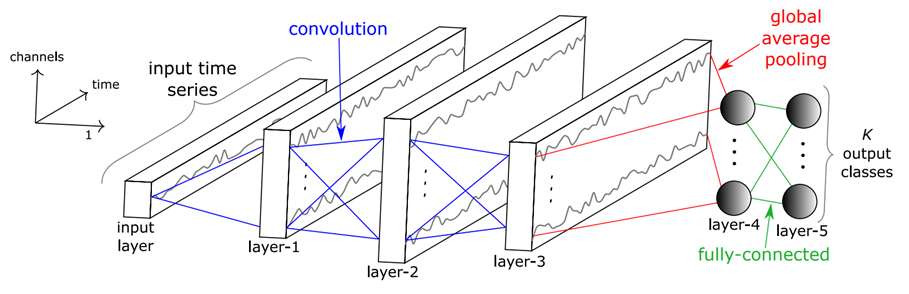
\includegraphics[width=1\linewidth]{FCN_struc.png}
    \caption{FCN Architecture}
    \label{fig:enter-label}
\end{figure}

\section{EVALUATION}
To evaluate the accuracy of the models, we use three parameters 
which are Root Mean Squared Error (RMSE), Mean Absolute Percentage Error (MAPE), Mean Squared Logarithmic Error (MSLE). The algorithm with the lowest value of those three parameters has the best performance. Below is the formula for RMSE, MAPE, and MSLE.

\begin{enumerate}
\item \textbf{Root Mean Squared Error (RMSE):}
\[RMSE = \sqrt{\frac{1}{n} \sum_{i=1}^{n} (y_i - \hat{y}_i)^2}\]
\item  \textbf{Mean Absolute Percentage Error (MAPE):}
\[MAPE = \frac{1}{n} \sum_{i=1}^{n} \left| \frac{y_i - \hat{y}_i}{y_i} \right| \times 100\%\]
\item \textbf{Mean Squared Logarithmic Error (MSLE):}
\[MSLE = \frac{1}{n} \sum_{i=1}^{n} (\log(1 + y_i) - \log(1 + \hat{y}_i))^2\]
\end{enumerate}

\section{RESULT}
\label{sec:guidelines}
\hspace{1em}In this section, we use the best performance (lowest error) model for each train/test ratio of each dataset to predict the next 30 days. 
\subsection{ACB}
\subsubsection{7:3 Train/Test ratio}
\begin{table}[H]
    \centering
    \begin{tabular}{|c|c|c|c|}
    \hline
    Model & \textbf{RMSE} & \textbf{MAPE} & \textbf{MSLE} \\
    \hline
    Linear Regression & 7914.5637 & 29.493 & 0.1508 \\
    \hline
    ARIMA & 5241.16 & 16.975 & 0.0549 \\
    \hline
    SVR & 12453.958 & 47.253 & 0.5152 \\
    \hline
    \rowcolor{red!10}
    LSTM & 665.57 & 2.186 & 0.0007 \\
    \hline
    VAR & 4531.319 & 14.287 & 0.0392 \\
    \hline
    Random Forrest & 6273.3679 & 23.4715 & 0.0829 \\
    \hline
    Seq2Seq & 736.9556 & 2.19 & 0.000961 \\
    \hline
    FCN & 1206.976 & 3.91 & 0.00234 \\
    \hline
    \end{tabular}
    \caption{7:3 ACB Ratio}
    \label{tab:my_label}
\end{table}

The best-suited model: LSTM model for 7:3 ACB
\begin{figure}[H]
    \centering
    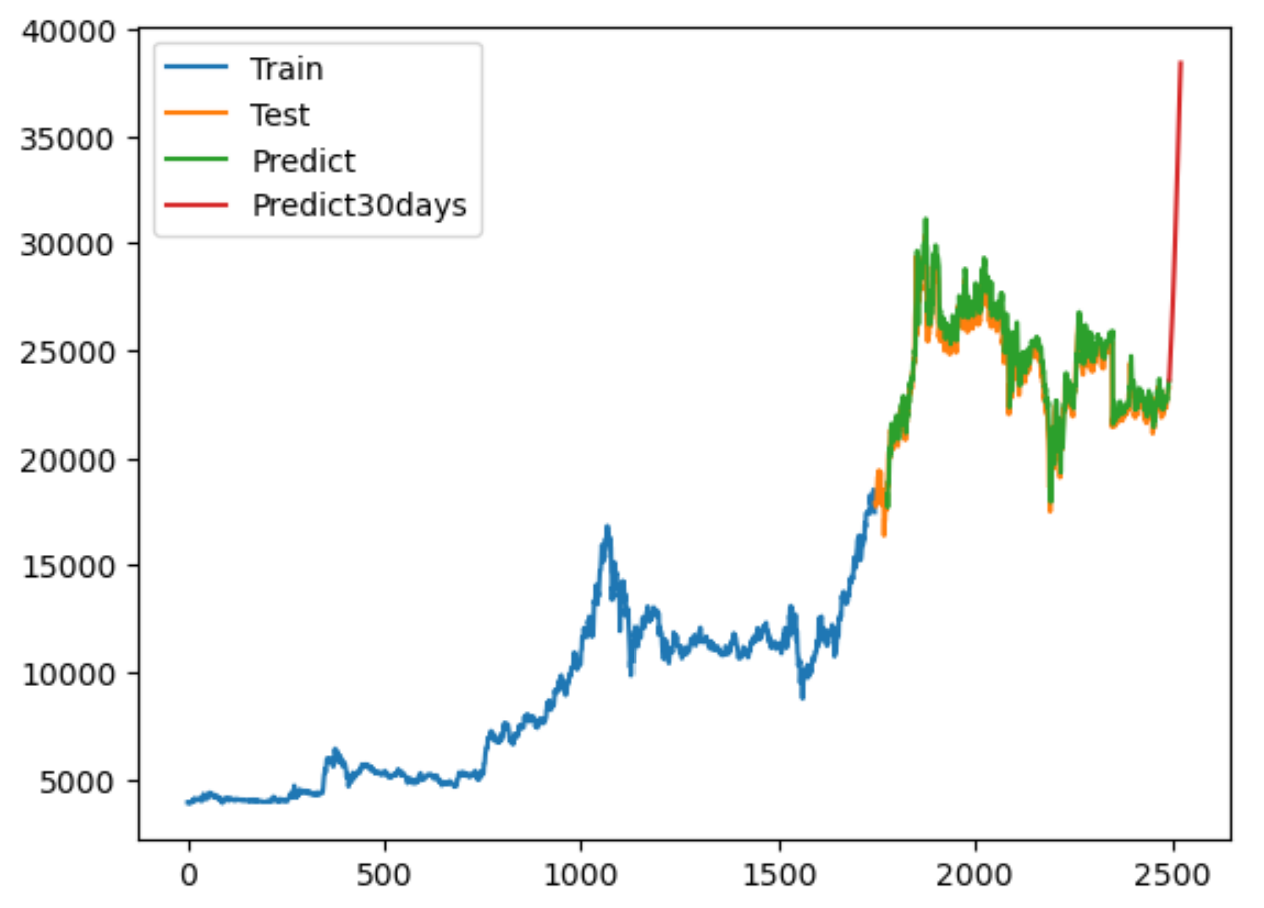
\includegraphics[width=1\linewidth]{acb_lstm_73.png}
    \caption{LSTM model}
    \label{fig:enter-label}
\end{figure}

\subsubsection{8:2 Train/Test ratio}
\begin{table}[H]
    \centering
    \begin{tabular}{|c|c|c|c|}
    \hline
    Model & \textbf{RMSE} & \textbf{MAPE} & \textbf{MSLE} \\
    \hline
    Linear Regression & 3245.4505 & 10.863 & 0.01932 \\
    \hline
    ARIMA & 5944.317 & 22.883 & 0.0526 \\
    \hline
    \rowcolor{red!10}
    SVR & 453.4623 & 1.265 & 0.00038 \\
    \hline
    LSTM & 500.7 & 1.464 & 0.0004 \\
    \hline
    VAR & 6337.585 & 24.557 & 0.0588 \\
    \hline
    Random Forrest & 858.3885 & 2.837 & 0.001329 \\
    \hline
    Seq2Seq & 726.2946 & 2.35 & 0.001004 \\
    \hline
    FCN & 1241.7439 & 4.45 & 0.002867 \\
    \hline
    \end{tabular}
    \caption{8:2 ACB Ratio}
    \label{8:2 VCB}
\end{table}
The best-suited model: SVR model for 8:2 ACB
\begin{figure}[H]
    \centering
    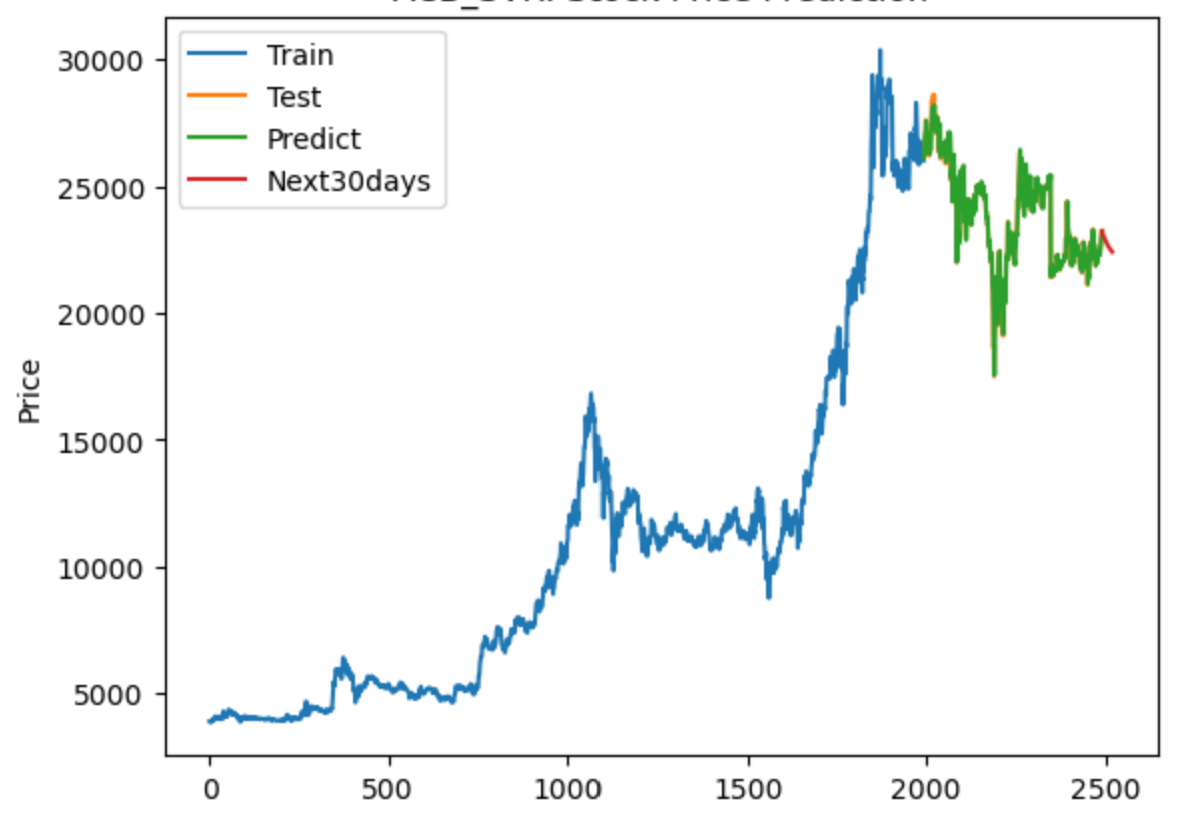
\includegraphics[width=1\linewidth]{acb_svr_82.png}
    \caption{SVR model}
    \label{fig:enter-label}
\end{figure}

\subsubsection{9:1 Train/Test ratio}
\label{subsec:9:1 VCB}
\begin{table}[H]
    \centering
    \begin{tabular}{|c|c|c|c|}
    \hline
    Model & \textbf{RMSE} & \textbf{MAPE} & \textbf{MSLE} \\
    \hline
    Linear Regression & 2609.8566 & 9.719 & 0.01197 \\
    \hline
    ARIMA & 1354.823 & 4.851 & 0.0033 \\
    \hline
    \rowcolor{red!10}
    SVR & 402.7491 & 1.00598 & 0.000292 \\
    \hline
    LSTM & 522.41 & 1.723 & 0.0005 \\
    \hline
    VAR & 1910.577 & 7.798 & 0.0066 \\
    \hline
    Random Forrest & 454.8253 & 1.289836 & 0.000385 \\
    \hline
    Seq2Seq & 563.8249 & 1.71 & 0.00059 \\
    \hline
    FCN & 1022.7937 & 3.50 & 0.001943 \\
    \hline
    \end{tabular}
    \caption{9:1 ACB Ratio}
    \label{tab:9:1 VCB}
\end{table}
The best-suited model: SVR model for 9:1 ACB

\begin{figure}[H]
    \centering
    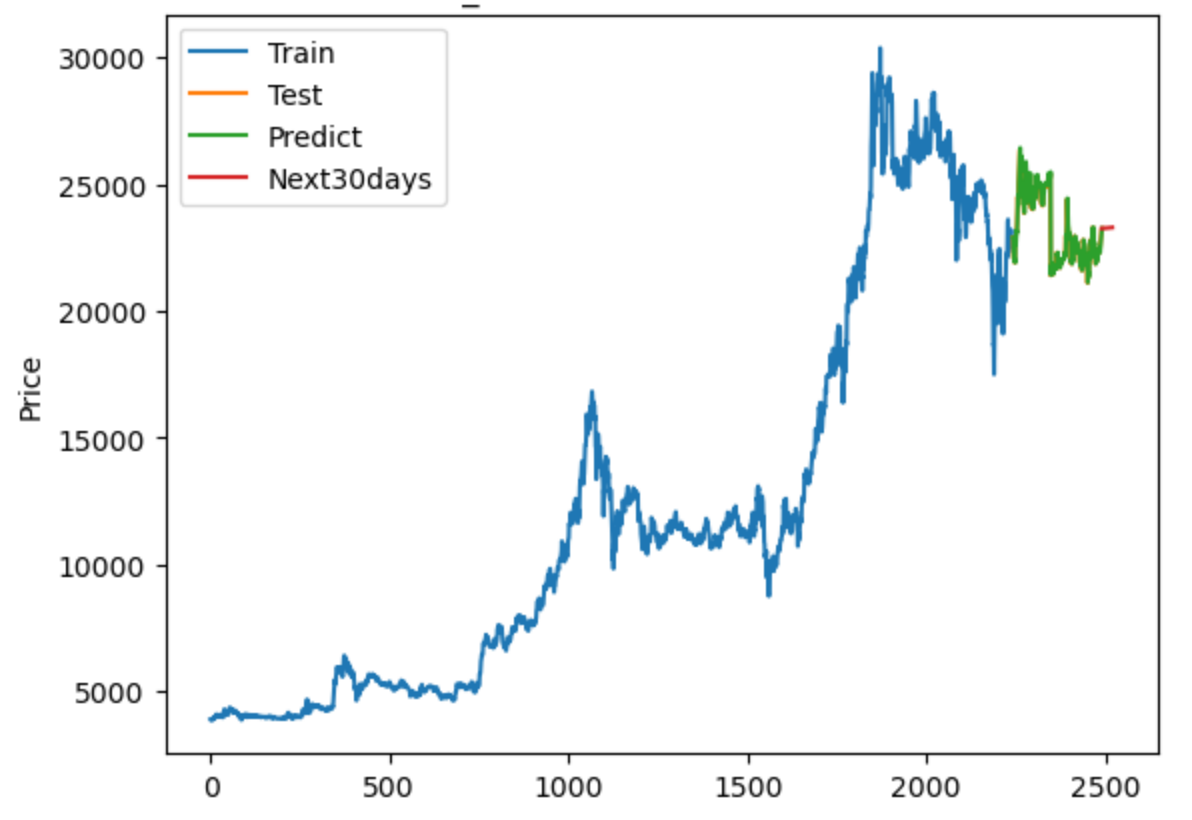
\includegraphics[width=1\linewidth]{acb_svr_91.png}
    \caption{SVR model}
    \label{fig:enter-label}
\end{figure}

\subsection{BIDV}
\subsubsection{7:3 Train/Test ratio}

\begin{table}[H]
    \centering
    \begin{tabular}{|c|c|c|c|}
    \hline
    Model & \textbf{RMSE} & \textbf{MAPE} & \textbf{MSLE} \\
    \hline
    Linear Regression & 3881.874 & 8.3104 & 0.01029 \\
    \hline
    ARIMA & 5273.644 & 12.038 & 0.0184 \\
    \hline
    SVR & 5500.5356 & 7.7549 & 0.01883 \\
    \hline
    LSTM & 1039.54 & 2.066 & 0.0007 \\
    \hline
    VAR & 6386.942 & 15.203 & 0.027 \\
    \hline
    Random Forrest & 2586.5432 & 4.3943 & 0.00368 \\
    \hline
    \rowcolor{red!10}
    Seq2Seq & 857.092 & 1.62 & 0.000506 \\
    \hline
    FCN & 1812.1182 & 3.80 & 0.00224 \\
    \hline
    \end{tabular}
    \caption{7:3 BIDV Ratio}
    \label{tab:my_label}
\end{table}
The best-suited model: Seq2Seq model for 7:3 BIDV
\begin{figure}[H]
    \centering
    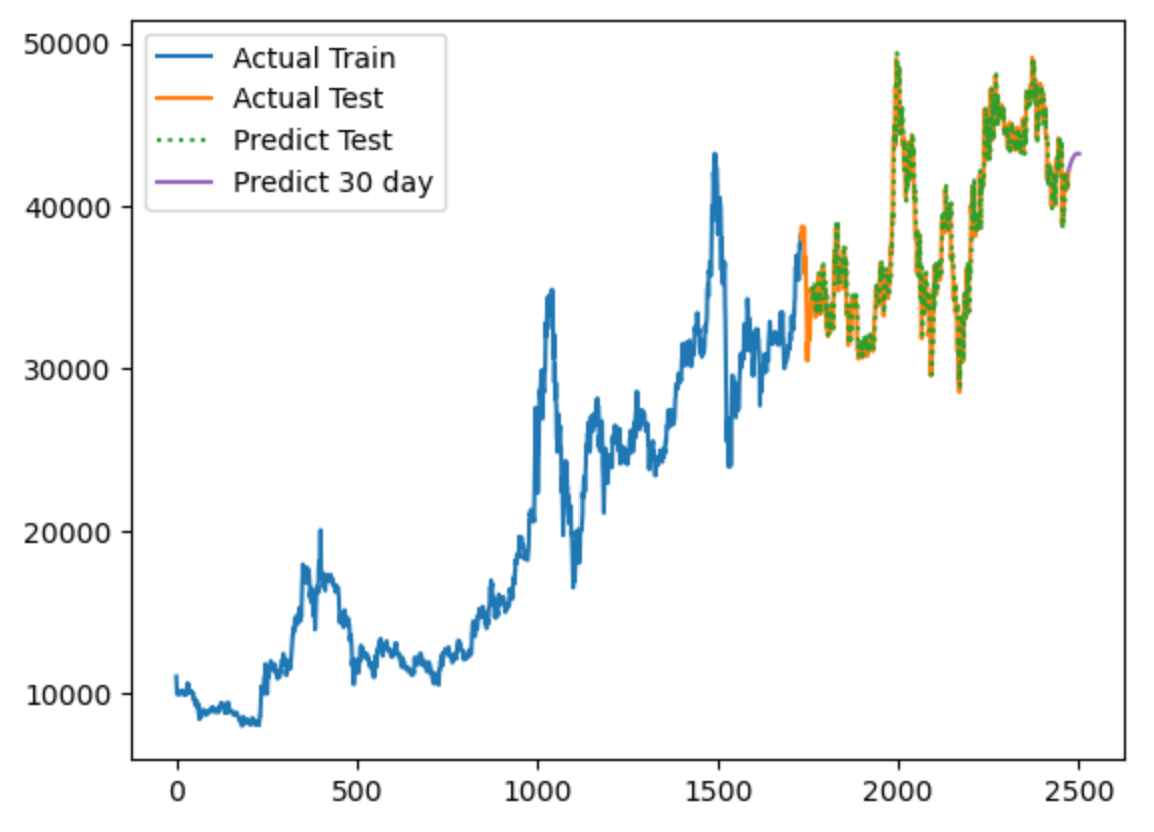
\includegraphics[width=1\linewidth]{bidv_s2s_73.png}
    \caption{Seq2Seq model}
    \label{fig:enter-label}
\end{figure}

\subsubsection{8:2 Train/Test ratio}
\begin{table}[H]
    \centering
    \begin{tabular}{|c|c|c|c|}
    \hline
    Model & \textbf{RMSE} & \textbf{MAPE} & \textbf{MSLE} \\
    \hline
    Linear Regression & 4379.2149 & 9.0322 & 0.01221 \\
    \hline
    ARIMA & 7547.189 & 15.115 & 0.0361 \\
    \hline
    SVR & 6203.97 & 10.201 & 0.02334 \\
    \hline
    LSTM & 927.69 & 1.746 & 0.0005 \\
    \hline
    VAR & 4998.594 & 9.926 & 0.0153 \\
    \hline
    Random Forrest & 1127.7548 & 1.91 & 0.000632 \\
    \hline
    \rowcolor{red!10}
    Seq2Seq & 905.8123 & 1.66 & 0.000554 \\
    \hline
    FCN & 1293.7144 & 2.56 & 0.001106 \\
    \hline
    \end{tabular}
    \caption{8:2 BIDV Ratio}
    \label{tab:my_label}
\end{table}
The best-suited model:  Seq2Seq model for 8:2 BIDV
\begin{figure}[H]
    \centering
    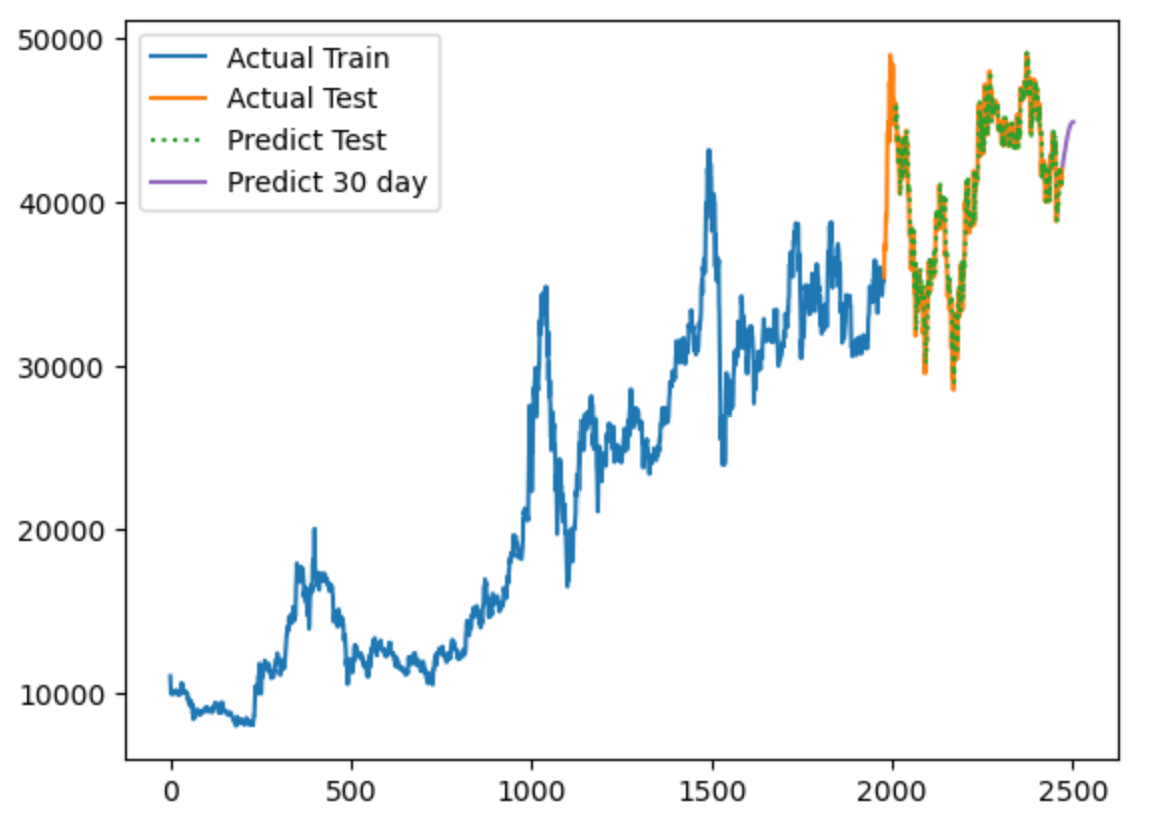
\includegraphics[width=1\linewidth]{bidv_s2s_82.png}
    \caption{Seq2Seq model}
    \label{fig:enter-label}
\end{figure}

\subsubsection{9:1 Train/Test ratio}
\begin{table}[H]
    \centering
    \begin{tabular}{|c|c|c|c|}
    \hline
    Model & \textbf{RMSE} & \textbf{MAPE} & \textbf{MSLE}\\
    \hline
    Linear Regression & 3572.8447 & 7.1005 & 0.00674 \\
    \hline
    ARIMA & 5854.336 & 12.034 & 0.0193 \\
    \hline
    SVR & 1493.611 & 2.44154 & 0.00109 \\
    \hline
    LSTM & 1429.35 & 2.841 & 0.001 \\
    \hline
    VAR & 3705.591 & 7.2904 & 0.0072 \\
    \hline
    Random Forrest & 1199.4247 & 2.0366 & 0.000711 \\
    \hline
    \rowcolor{red!10}
    Seq2Seq & 739.4482 & 1.17 & 0.000284 \\
    \hline
    FCN & 964.1519 & 1.62 & 0.000489 \\
    \hline
    \end{tabular}
    \caption{9:1 BIDV Ratio}
    \label{tab:my_label}
\end{table}
The best-suited model: Seq2Seq model for 9:1 BIDV
\begin{figure}[H]
    \centering
    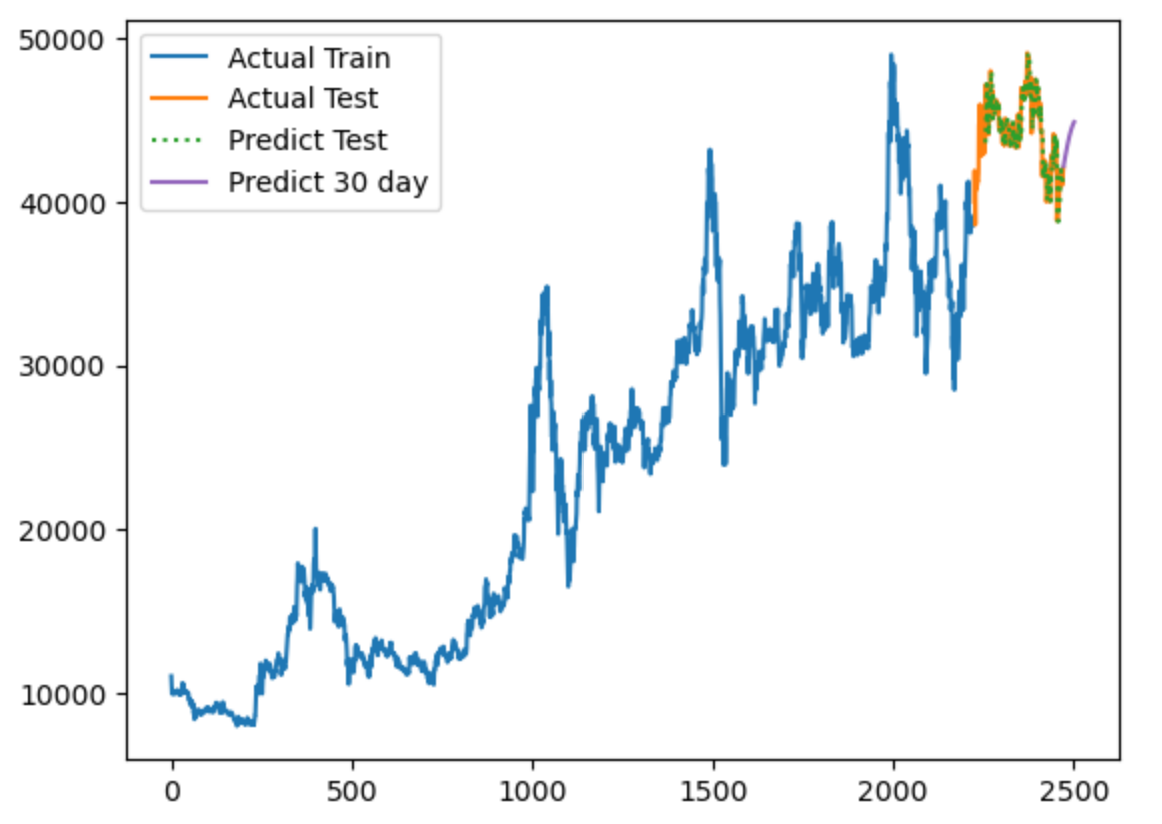
\includegraphics[width=1\linewidth]{bidv_s2s_91.png}
    \caption{Seq2Seq model}
    \label{fig:enter-label}
\end{figure}


\subsection{VCB}
\subsubsection{7:3 Train/Test ratio}

\begin{table}[H]
    \centering
    \begin{tabular}{|c|c|c|c|}
    \hline
    Model & \textbf{RMSE} & \textbf{MAPE} & \textbf{MSLE} \\
    \hline
    Linear Regression & 7481.893 & 7.4121 & 0.00864 \\
    \hline
    ARIMA & 9723.279 & 9.89 & 0.013 \\
    \hline
    SVR & 24611.323 & 21.92 & 0.1225 \\
    \hline
    LSTM & 2283.62 & 2.327 & 0.0007 \\
    \hline
    VAR & 9684.298 & 9.829 & 0.0129 \\
    \hline
    Random Forrest & 10069.8906 & 8.2158 & 0.01429 \\
    \hline
    \rowcolor{red!10}
    Seq2Seq & 1841.9644 & 1.64 & 0.000496 \\
    \hline
    FCN & 2817.4579 & 2.0 & 0.001133 \\
    \hline
    \end{tabular}
    \caption{7:3 VCB Ratio}
    \label{tab:my_label}
\end{table}
The best-suited model: Seq2Seq model for 7:3 VCB
\begin{figure}[H]
    \centering
    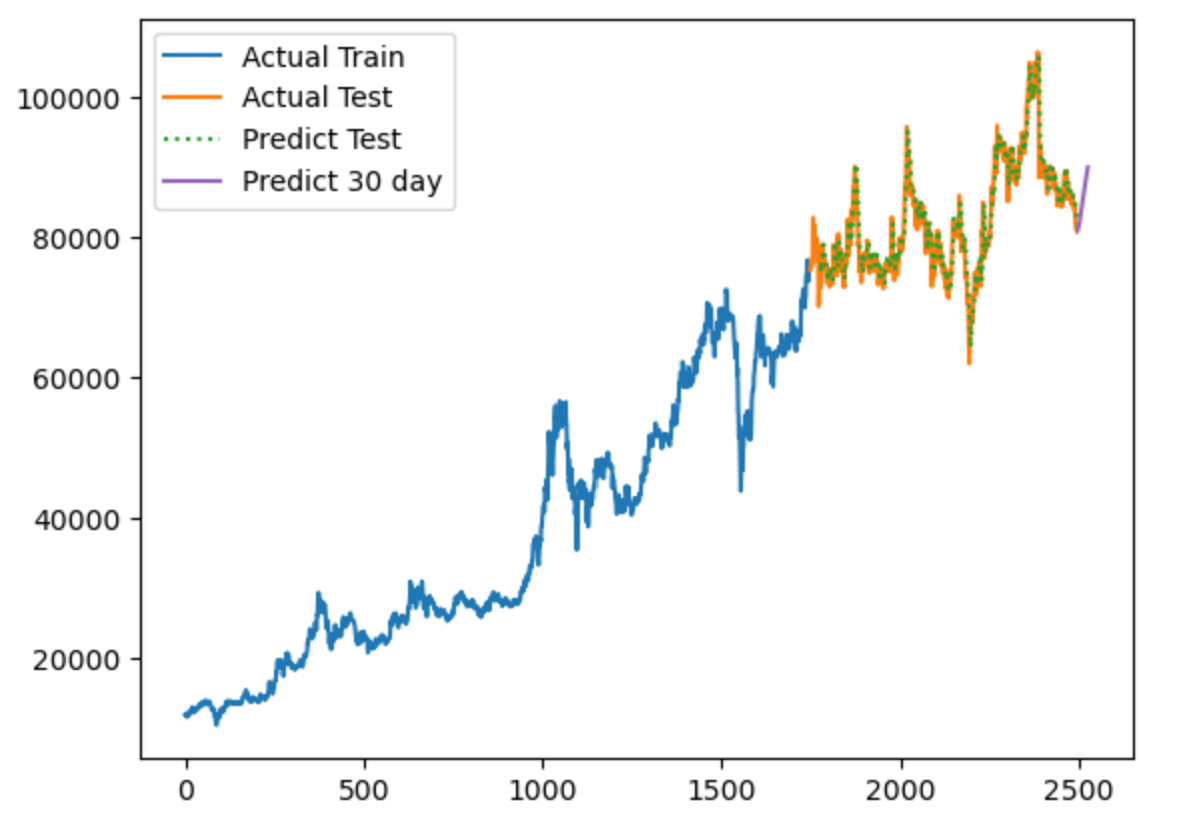
\includegraphics[width=1\linewidth]{vcb_s2s_73.png}
    \caption{Seq2Seq modelmodel}
    \label{fig:enter-label}
\end{figure}

\subsubsection{8:2 Train/Test ratio}
\begin{table}[H]
    \centering
    \begin{tabular}{|c|c|c|c|}
    \hline
    Model & \textbf{RMSE} & \textbf{MAPE} & \textbf{MSLE} \\
    \hline
    Linear Regression & 7562.7874 & 7.5426 & 0.00818 \\
    \hline
    ARIMA & 7467.38 & 6.853 & 0.0076 \\
    \hline
    SVR & 13616.361 & 9.815 & 0.02771 \\
    \hline
    \rowcolor{red!10}
    LSTM & 1642.38 & 1.3701 & 0.0003 \\
    \hline
    VAR & 7200.996 & 6.963 & 0.0073 \\
    \hline
    Random Forrest & 4751.289 & 3.149 & 0.00265 \\
    \hline
    Seq2Seq & 2068.8175 & 1.77 & 0.000606 \\
    \hline
    FCN & 2728.555 & 2.47 & 0.001055 \\
    \hline
    \end{tabular}
    \caption{8:2 VCB Ratio}
    \label{tab:my_label}
\end{table}
The best-suited model: LSTM model for 8:2 VCB
\begin{figure}[H]
    \centering
    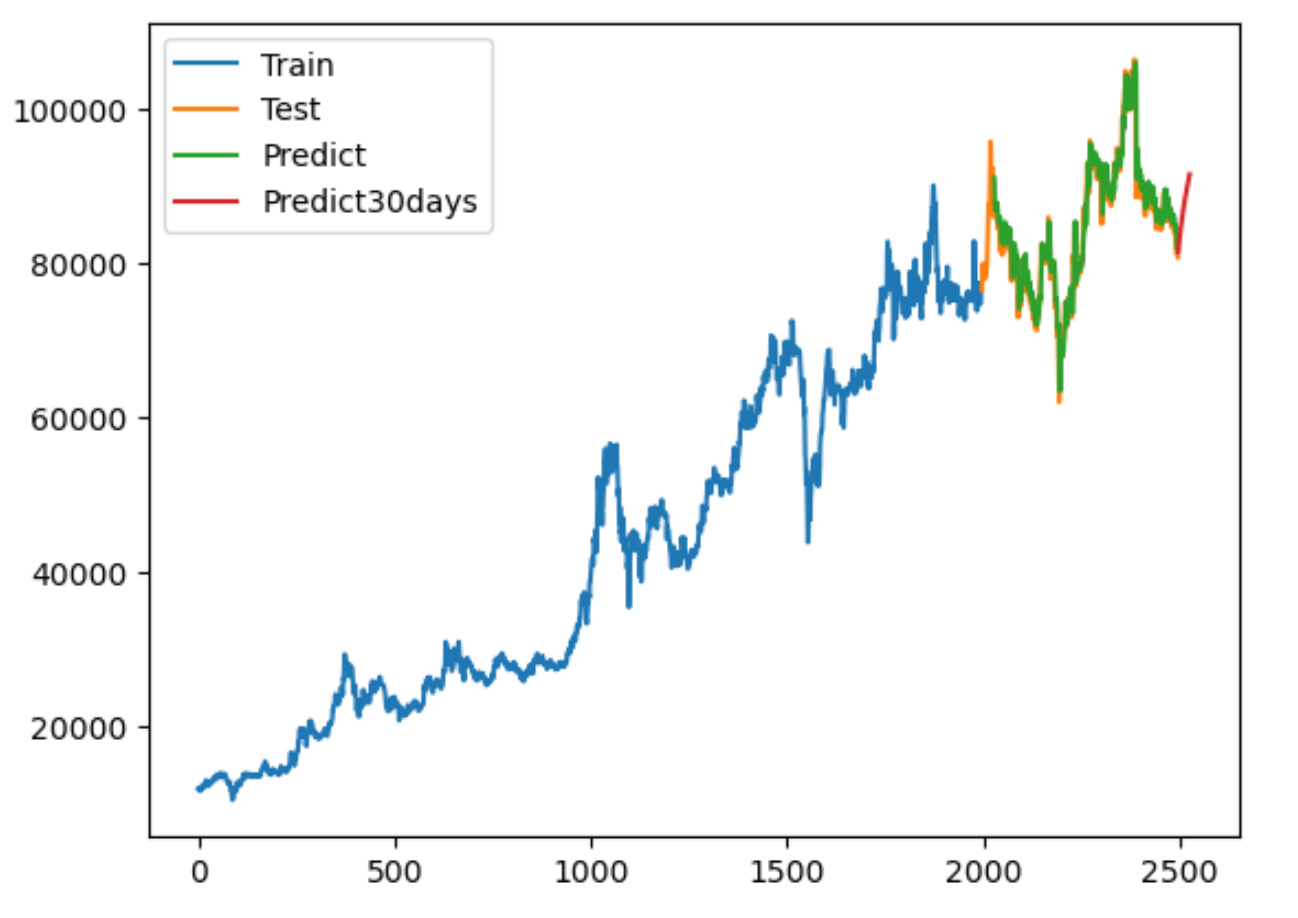
\includegraphics[width=1\linewidth]{vcb_lstm_82.png}
    \caption{LSTM modelmodel}
    \label{fig:enter-label}
\end{figure}

\subsubsection{9:1 Train/Test ratio}
\begin{table}[H]
    \centering
    \begin{tabular}{|c|c|c|c|}
    \hline
      Model & \textbf{RMSE} & \textbf{MAPE} & \textbf{MSLE} \\
        \hline
        Linear Regression & 7562.7874 & 7.5426 & 0.00818 \\
        \hline
        ARIMA & 9968.438 & 8.484 & 0.0124 \\
        \hline
        SVR & 11241.226 & 8.32024 & 0.016302 \\
        \hline
        \rowcolor{red!10}
        LSTM & 1615.53 & 1.099 & 0.0002 \\
        \hline
        VAR & 10112.09 & 8.643 & 0.0128 \\
        \hline
        Random Forrest & 5611.5296 & 3.98 & 0.003508 \\
        \hline
        Seq2Seq & 2061.942 & 1.45 & 0.000481 \\
        \hline
        FCN & 2689.939 & 2.13 & 0.000819 \\
        \hline
    \end{tabular}
    \caption{9:1 VCB Ratio}
    \label{tab:my_label}
\end{table}
The best-suited model: LSTM model for 9:1 VCB
\begin{figure}[H]
    \centering
    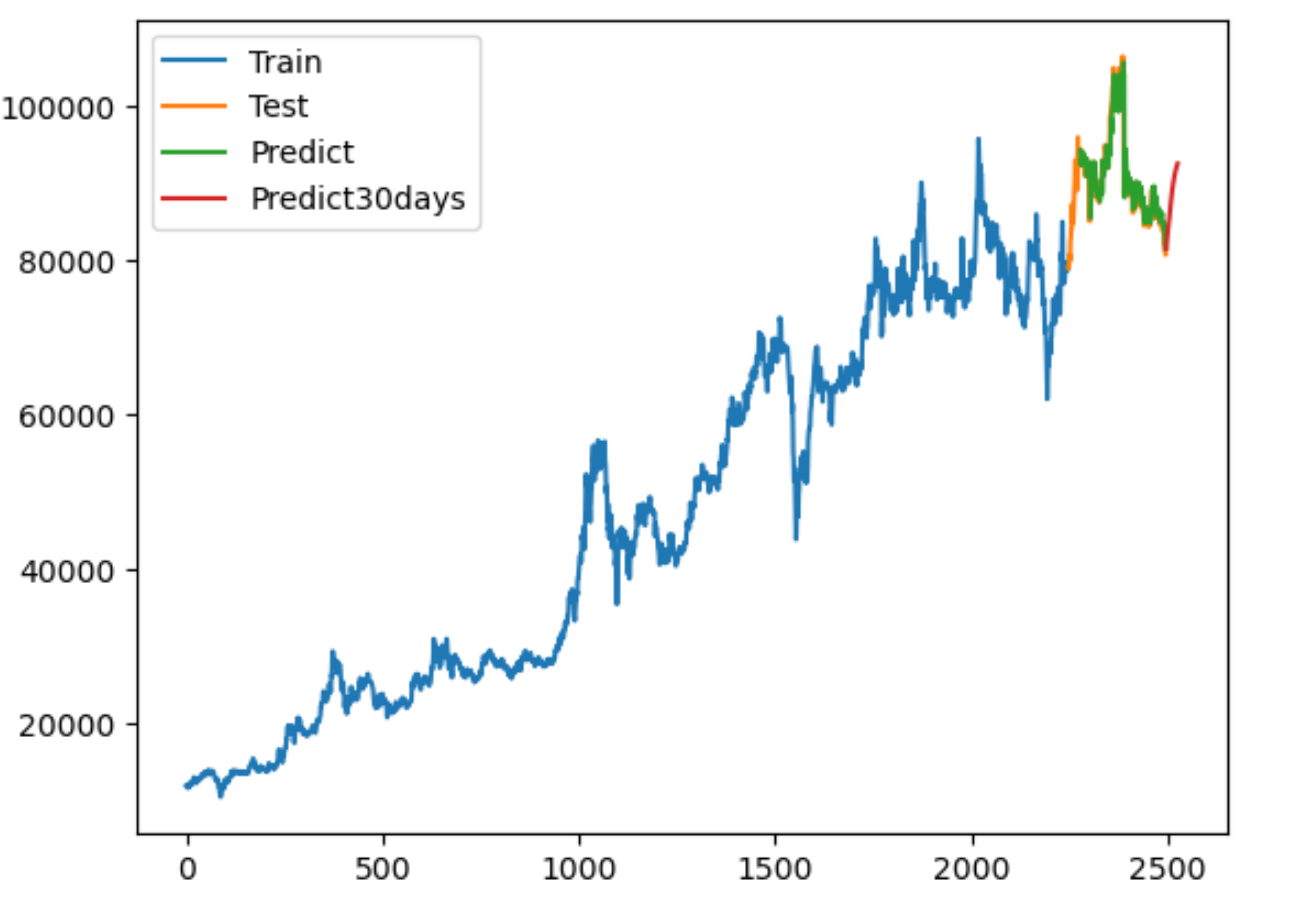
\includegraphics[width=1\linewidth]{vcb_lstm_91.png}
    \caption{LSTM model}
    \label{fig:enter-label}
\end{figure}

\section{Conclusion}
\hspace{1em}The utilization of LSTM and seq2seq models to predict the stock prices of major banks in Vietnam such as ACB, VCB, and BIDV has demonstrated substantial potential in learning and generating forecasts based on the learned models alongside the other models used in this project (Linear Regression, ARIMA, SVR, LSTM, VAR, Random Forest, Seq2Seq, FCN). Both of these models exhibit the capability to handle time series data and learn intricate relationships within the sequences.

Assessing the stock price predictions for the upcoming 30 days using these models, both LSTM and seq2seq indicate a slight upward trend in the future stock prices of these banks. However, evaluating the "suitability" of a model for predicting an upward trend relies not only on its predictive capability but also on a profound understanding of the financial market and the fine-tuning and optimization of the model.

Hence, it's crucial to note that the accuracy of predictions does not solely stem from the model but also hinges on the harmonious integration of the model with domain expertise and the process of adjusting the model for effective real-world applications. 

\section{Orientation}
\hspace{1em}Our current models may not be entirely accurate, and it is essential to allocate time for validating real-world predictions made by these models. Errors within the models might arise from research limitations or inappropriate model selection concerning the datasets used. Hence, there is room for further improvement in our models for the future.

For instance, enhancing existing models could involve integrating attention mechanisms into Seq2Seq models. This addition enables a focus on crucial parts of the input sequence, thereby enhancing the transformation from input to output data. Additionally, combining LSTM with other architectures like Convolutional Neural Networks (CNNs) or Attention Mechanisms could yield more robust models.

Furthermore, we plan to explore other models such as Transformers and various Gradient Boosting methods to compare their performance with our current models in practical scenarios. This comparative analysis aims to identify the most suitable model for our purposes.

In conclusion, our strategy involves both enhancing existing models and exploring new ones to improve accuracy and efficacy in real-world applications.

\section*{Acknowledgment}
\hspace{1em}We extend our heartfelt appreciation to Assoc. Prof. Dr. Nguyen Dinh Thuan and TA. Nguyen Minh Nhut for their invaluable expertise and wholehearted guidance throughout this project. Without your passionate supervision, our group's report would have been incredibly challenging to complete.

This project has provided an excellent opportunity for each team member to collaborate, enhance their cooperative skills, exchange knowledge, and, significantly, put theoretical learning into practical application.

Throughout the project's execution, the team effectively utilized the taught knowledge while embracing new concepts, aspiring to achieve perfection in our work. Nevertheless, due to constraints such as time, limited knowledge, and experience, shortcomings are inevitable. Hence, the group eagerly anticipates receiving your valuable suggestions. These insights will aid in augmenting our understanding and skills, enabling us to contribute better to future projects and real-world scenarios.

Lastly, our team wishes you continued good health to persist in your noble endeavor of imparting knowledge to the upcoming generations.

\bibliographystyle{plain}
\bibliography{reference}
\EOD

\end{document}
